% !Mode:: "TeX:UTF-8"

\chapter[绪论]{绪论}[]

\label{chap:1}

\section{研究背景及意义}

\subsection{研究背景}

深度神经网络在计算机视觉领域的诸多基准任务上取得了令人瞩目的成绩，ImageNet、COCO 等大规模标注数据上的识别精度接近甚至超越人类水平，但其性能突破的背后隐含着一个常被忽视的前提：训练数据与测试数据服从独立同分布~\cite{liang2021source}。在真实部署中，目标侧条件可能在数据分布、类别词表或任务语义要求上偏离训练条件，由此引发三类在抽象层次上逐级递进的稳健性问题。图~\ref{fig:iidood} 对比了三类变化下的训练条件、目标条件及模型所需能力。

\begin{figure}[!htbp]
 \centering
 \includegraphics[width=.8\linewidth]{figures/multi_generalization_shift.pdf}
 \bicaption[fig:iidood]{}{训练与目标条件在数据分布、类别词表和语义要求上的差异}{Fig.}{Differences between training and target conditions in data distribution, category vocabulary, and semantic requirements}
\end{figure}

数据分布维度的失配是最直观且被研究最为广泛的一类稳健性问题。深度神经网络在训练过程中习得的并非纯粹的类别语义表征，而是将语义信息与源域的纹理风格、光照条件、采集设备特征等多层次信息深度纠缠地编码于同一特征空间~\cite{ganin2016domain,long2015learning}。这种纠缠根源于经验风险最小化在独立同分布假设下对源域损失的直接优化。过参数化的网络倾向于记忆源域样本的表面统计而非学习真正可泛化的语义不变特征，使得跨域时分类器权重所定义的判别方向在源域最优而在目标域系统性偏移。这种偏移进一步导致模型在目标域的预测不仅精度下降，还伴随显著的高置信度错误风险，例如softmax 输出对未知样本仍给出接近 1.0 的伪置信，使决策难以被阈值过滤或人工干预~\cite{liang2021source,yang2021neighbor}。在更严苛的无源设定下，源域数据因隐私法规、商业机密或存储成本等约束不可访问，模型需在源数据完全缺位的条件下仅凭源模型参数中编码的知识完成跨域传递，而由于深度特征的纠缠本质，我们无法从模型参数中直接辨识哪些知识可迁移、哪些是源域特定的虚假相关，进一步加剧了迁移的不确定性，所以就需要结合目标域数据进一步做不确定分析。
本文将这种需要将模型部署到数据分布偏移的场景称之为“域泛化”场景，与文献~\cite{zhou2023domain}中特指模型在源域完成泛化而部署时完全不接触任何目标数据的域泛化设定在前提假设上并不等同。

类别词表维度的失配是另一类广泛存在却长期被低估的稳健性问题。传统深度分类器在架构层面预设了闭集假设，即分类头的输出维度等于训练类别数，其判别性表征也是在固定类别索引上优化得到的~\cite{radford2021learning}。这一架构选择带来双重约束：一方面，分类头的权重矩阵与固定的 N 个类别索引强绑定，新类别没有对应的输出通道；另一方面，骨干网络针对 N 类判别任务优化，并未在特征空间中为未知类别预留结构化空间~\cite{kundu2022towards}。当目标场景的类别集合发生扩展、缩减或漂移时，分类头的维度结构与新类别空间在维度上不再兼容，已训练模型的判别能力在新类别上无法直接复用，并倾向于将未知样本强行归入概率最高的已知类别，产生高置信度的错误预测。这一现象在自动驾驶、工业质检等在线服务场景中尤为危险~\cite{kirillov2023segment}。为缓解这一约束，基于图文对比预训练的开放词汇分类器通过引入语言空间的语义先验扩展了类别边界，但其语义覆盖仍受限于预训练文本编码器的词表，难以覆盖长尾、新兴或专业领域类别~\cite{radford2021learning}。逐类重新采集、专家标注并重训模型的过程伴随显著的时间与资金投入，在隐私敏感与不可中断的业务场景中，这种``重训窗口''往往根本不可行~\cite{kirillov2023segment}。这要求识别模型能够在训练时未见过的新类别上完成判别，而传统固定词表架构在维度不兼容的设定下难以直接扩展，尤其在像素级分割任务中，新类别的精细空间定位对像素级标注成本与模型先验的开放语义能力同时提出要求，使类别词表维度的失配在通用识别研究中成为一个关键挑战。

语义层次维度的失配是相较前两者更高阶的稳健性问题。现有视觉基础模型（特别是多模态大语言模型）的预训练以事实型图文描述为主，习得的表征擅长回答“图像中有什么”这类可枚举的类别问题~\cite{mmbench2023}，却对隐含于视觉元素与文化语境、风格表征、符号解读之间的关联缺乏结构化编码，其流畅的语义表述多源于训练语料的统计相关而非基于视觉证据的可靠推理~\cite{achlioptas2021artemis,zhao2014exploring}。具体而言，预训练语料中的图像描述通常以物体、场景、动作等可枚举事实为骨架，而高阶情感与文化推理所需的细粒度证据化标注（如“左上方冷色笔触营造孤寂氛围”）在大规模数据中极为稀缺~\cite{aesexpert2024}，导致模型缺乏从局部视觉元素到整体情感语义的可追溯推理路径，其生成结果常表现为“流畅的虚构”——语言流畅、符合人类表达习惯，但缺乏对具体视觉元素的精确指涉~\cite{eemobench2025}。当识别任务从事实判断升级到“图像为何传达某种情感”、“差异由哪些视觉线索驱动”等需要感知能力与文化语境相融合的高阶推理时，模型所依赖的不再是可枚举的类别标签或显式物体事件，而是隐含在视觉元素与文化符号之间的语义关联。以艺术图像的情感推理为例，情感表达隐含于构图、笔触、风格化与文化符号之中，不同艺术流派的笔触技法与色彩配置所引发的情感反应具有显著的领域特异性~\cite{yang2023emoset}。然而现有通用多模态大语言模型评测基准多聚焦于事实识别层面~\cite{mmbench2023}，缺乏面向情感理解与证据化推理的结构化诊断协议，使得流畅的情感表述与基于视觉证据的可靠解释难以被精准区分~\cite{eemobench2025}，阻碍了视觉基础模型在高阶语义推理方向上的能力迭代。

综上，本文将模型在数据分布、类别词表或任务语义要求发生变化时仍需保持相应能力的这类情形统称为多泛化场景。三类变化分别要求模型维持跨域判别能力、识别未见类别，以及在事实识别之外完成有视觉证据支撑的高阶语义解释。本文从变化维度、目标侧条件和模型载体三个方面刻画这些场景：变化维度包括数据分布、类别词表与任务语义要求；目标侧条件包括无标签数据、有限人工标注，以及仅用于评测的目标任务样本；模型载体包括判别式视觉模型与多模态大语言模型（Multimodal Large Language Model, MLLM）。前两类研究通过目标域适应或跨模型融合改善迁移表现；第三类研究在不更新模型的条件下，以系统评测诊断已有能力面对更高层级语义任务时的适用范围与失效环节。
% 纯评测在此是研究方式，并非与无标注、少量标注并列的监督强度。

围绕上述多泛化场景，本文沿域泛化、类泛化与语义理解泛化三个层面展开研究。域泛化以数据分布变化为核心，面向判别式视觉模型在无标注或少量标注条件下的可靠迁移：前者通过伪标签去噪和鲁棒表征学习抑制迁移过程中的误差累积，后者利用多模态先验引导主动样本选择，以有限标注获得更高效的适应收益。类泛化进一步关注类别词表的开放变化，结合多模态先验与多基础模型协同，提升对新颖类别的识别和像素级定位能力。语义理解泛化则关注目标任务由事实识别扩展至情感归因与证据化解释时，MLLM 已有能力能否适用；本文通过多层级评测协议刻画其表现与失效环节，而不将评测结果解释为模型优化后的迁移增益。


\subsection{研究意义}
多泛化场景下的模型迁移，体现为研究对象从样本表征、类别概念到高阶语义的逐步拓展。数据分布维度（对应域泛化）关注像素风格、成像条件与统计特性的变化，核心在于学习具有跨域稳定性的表征；类别词表维度（对应类泛化）关注模型对未见类别的语义覆盖能力，核心在于实现开放环境下的识别与泛化；语义层次维度（对应语义理解泛化）关注模型能否超越事实层面的对象判别，完成情感归因、证据关联与高阶推理。
随着目标条件由分布变化扩展到类别开放，再到语义理解要求提升，模型所需保持的能力也从稳定判别延伸至新类识别与证据化解释。这一由表征到概念、再到语义的研究主线，既贯穿本文各章，也为复杂开放环境下的模型适应与能力评测提供了共同的问题框架。

\noindent\textbf{（1）域泛化方面} 

模型能否将训练阶段获得的知识有效迁移至分布不同的目标域，是迁移学习长期关注的核心问题~\cite{liang2021source,ganin2016domain,long2015learning}。棘手的是，深度表征中所蕴含的可迁移成分与域特异性成分在缺乏显式分解机制的条件下彼此纠缠，仅靠目标域自监督信号难以可靠地区分二者，伪标签噪声放大与判别性偏移是这一困境在方法层面的集中体现~\cite{yang2021neighbor,kundu2022towards}。同时，受数据隐私、版权保护和传输成本等现实因素影响，源域样本往往难以获取，使迁移过程中的可靠性诊断更具挑战。因此，研究源数据受限乃至不可访问条件下的可靠迁移机制，一方面有助于深化对无源域适应和少监督域适应中伪标签去噪、有效样本选择与鲁棒表征学习机制的认识；另一方面也能够为面向真实部署环境的目标域特征学习与高效适应策略提供方法依据。

\noindent\textbf{（2）类泛化方面} 

视觉识别系统在实际应用中面对的不再是封闭且预定义的类别集合，而是持续扩展的开放词汇空间。新物体、新材质、新场景不断涌现，固定训练词表及其对应的分类决策边界班一覆盖开放环境中的识别需求~\cite{kirillov2023segment,radford2021learning}。当模型遭遇训练阶段未见的类别时，往往会将其错误归入已有类别，并产生高置信度预测~\cite{kundu2022towards}。由此，开放词汇视觉识别的关键在于缓解封闭训练词表与开放识别需求之间的结构性错配。研究如何在缺乏目标类别标注的条件下发挥多模态基础模型的开放语义先验，并构建异质模型之间的协同机制，有助于揭示语义知识与空间定位知识的互补规律。这不仅能够为开放词汇分类、检测和分割模型的设计提供方法支撑，也有望降低模型适应新类别时对大规模重新训练和人工标注的依赖。

\newpage
\noindent\textbf{（3）语义理解泛化方面} 

多模态大语言模型已在多类事实型视觉识别任务中展现出较强能力，但在情感、意图、文化语境和审美判断等高阶语义任务中，其能力边界仍有待系统刻画~~\cite{mmbench2023,achlioptas2021artemis,eemobench2025}。这一挑战的深层原因在于：模型的预训练语料以可枚举的事实型图文描述为主，缺乏将局部视觉元素与整体情感语义相连接的可追溯推理路径~\cite{zhao2014exploring,aesexpert2024}；其语言流畅性往往源于训练统计相关而非视觉证据支撑~\cite{eemobench2025}。构建面向高阶视觉语义的基准化评测协议，是模型迁移研究在纯评测条件下的重要延伸：当目标任务缺少可用于进一步训练的监督信息时，评测能够刻画和诊断模型既有知识能否有效迁移至新的语义理解任务。此类评测不仅可为多模态大语言模型的能力诊断和后续优化提供量化依据，也有助于揭示视觉智能从感知走向认知仍然缺失的关键能力，从而推动视觉基础模型向更可靠、更具证据支撑的高阶语义推理发展。将高阶语义理解沿感知、情感、推理与描述四个多维互补层级分别考察，使语义层面的能力边界既可被定位也可被比较。

\section{国内外研究现状}

\subsection{面向域泛化场景的跨域不变特征学习}

真实场景中的光照、拍摄设备、视角和图像风格会随环境变化，使同一类别的目标呈现不同外观。域适应研究因此关注：模型能否在这些变化下保留与类别相关的判别信息，避免过度依赖特定数据域中的背景或纹理。本节所讨论的跨域不变特征学习，正是指在源域与目标域分布不同时，学习仍能支持目标域识别的视觉表征。

跨域不变性的实质是使特征对域的变化保持不敏感：同一类别的样本无论来自哪个域，都应保留与类别相关的判别结构，而不被特定域的背景、纹理与风格所主导。这一性质能否成立，既取决于模型能否构造出跨域可用的监督信号，也取决于骨干网络能否在特征生成阶段即削弱域偏移的影响。
基于上述分析，域适应研究相应地在迁移机制与骨干架构两个方向上积累了工作，前者包含分布对齐、自训练及有限标注的利用，决定模型如何借助可用数据适应目标域；后者涉及模型对局部细节与长程依赖的建模方式，影响跨域不变特征的捕获能力。下面先梳理无监督设定下的迁移机制与骨干架构演进，再讨论监督信号稀缺时相关机制的发展。

\subparagraph{无监督域适应方法}

无监督模型迁移中的不确定性，是指源域模型面对目标域分布变化、且缺乏目标标签校验时，特征表征与预测结果的可靠性难以保证。它既可能来自模型对源域纹理、背景等域特异性线索的依赖，也可能表现为目标样本预测或聚类结果的不稳定。伪标签噪声是这种不确定性在自训练监督环节的具体表现。当错误预测被当作目标域标签反复用于更新，误差便可能进一步改变特征空间，导致后续伪标签继续偏移。因此，不确定性抑制需要同时关注监督信号是否可信，以及产生该信号的表征是否稳定。

无监督域适应（Unsupervised Domain Adaptation, UDA）方法按其核心机制可划分为五大类：基于领域分布差异对齐的方法~\cite{sun2016deep,chen2019maximum}，通过度量并最小化源域与目标域在特征空间或像素空间的分布距离实现跨域对齐；基于对抗的方法DANN~\cite{ganin2016domain}，借助域判别器引导特征提取器生成域不变表征；基于重构的方法~\cite{ghifary2016deep,bousmalis2017domain}，通过图像或特征重构分解域相关与类相关成分；基于样本生成的方法~\cite{sankaranarayanan2018generate}，借助生成对抗网络或扩散模型合成目标域风格样本以缓解域偏移；以及基于自学习的方法~\cite{SRDC,SimNet,xie2018unsupervised}，其核心思想是通过源域标签样本引导，为无标签目标样本分配伪标签，再以迭代自训练或聚类方式进行精炼。具体而言，SRDC~\cite{SRDC} 通过判别性聚类揭示目标数据的内在结构；SimNet~\cite{SimNet} 通过类别原型相似度进行分类；Xie 等人~\cite{xie2018unsupervised} 进一步将自训练与样本加权相结合。上述五类方法均依赖源域训练样本在适应阶段持续可访问，构成了无监督域适应方法的主体谱系。

\begin{figure}[!htbp]
    \setlength{\tabcolsep}{0pt}
    \centering
    \subfigure[DANN框架图~\cite{DANN}]{%
    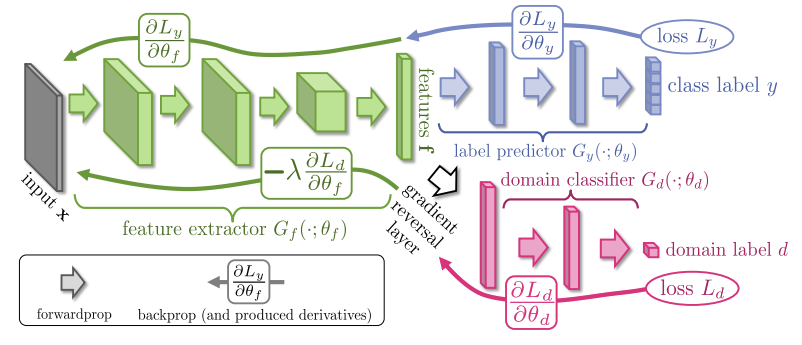
\includegraphics[width=0.48\linewidth]{figures/related_work/DANN.png}%
    }\hfill
    \subfigure[SHOT机制~\cite{liang2021source}]{%
    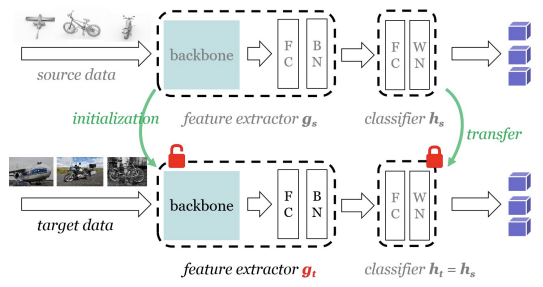
\includegraphics[width=0.48\linewidth]{figures/related_work/SHOT.png}%
    }
    \bicaption[fig:da_works]{}{域迁移代表方法}{Fig.}{Representative methods for domain adaptations}
\end{figure}

在 UDA 方法谱系之上，进一步收紧至“源数据不可访问”这一严格设定，即得到无源域适应（Source-Free Domain Adaptation, SFDA）~\cite{liang2021source}。该设定下，原有方法所依赖的源数据统计量、域判别信号、跨域重构样本与伪标签生成机制均无法直接调用，必须在仅有源模型参数的条件下构造新的跨域监督。源假设迁移（Source-Hypothesis Transfer, SHOT）~\cite{liang2021source} 通过冻结源分类器对目标特征聚类生成伪标签，成为该方向的开创性工作；NRC~\cite{yang2021neighbor} 利用邻居关系约束类内一致性；CoWA-JMDS~\cite{cowa}、U-SFAN~\cite{U-SFAN} 引入模型不确定性或数据不确定性估计对伪标签进行加权；D-MCD~\cite{chu2022denoised} 通过双分类器对抗训练识别高置信度样本中的噪声；VDM-DA~\cite{tian2022vdm} 借助虚拟域判别器选择熵值较低的干净伪标签；SSNLL~\cite{chen2022self} 以指数滑动平均模型对样本进行分层处理；Kundu 等人~\cite{kundu2022towards} 进一步从信息瓶颈角度给出 SFDA 目标风险的显式上界，为上述方法提供理论解释。


骨干网络的设计深刻影响实例级跨域不变特征的捕获能力，呈现出从 CNN 局部感受野到 ViT 全局注意力、再到选择性扫描状态空间模型（State-Space Model, SSM）Mamba 线性长程建模的清晰演进脉络。CNN（尤其是 ResNet~\cite{he2016deep}）凭借层次化特征聚合的归纳偏置~\cite{yang2021neighbor,xia2021adaptive,zhang2024nami}，是大量域迁移的默认选择；然而固定局部感受野难以捕获跨区域对象结构关系~\cite{long2015learning,ganin2016domain}。针对这一局限，ViT~\cite{dosovitskiy2021image} 通过自注意力机制实现全局感受野~\cite{sanyal2023stable,xia2024dual}，DSIT~\cite{sanyal2023dsit}、TransDA~\cite{TransDA}、C-SFTrans~\cite{sanyal2024aligning}、DPC~\cite{dpc} 等工作将 ViT 引入域适应；但 $\mathcal{O}(N^2)$ 的注意力复杂度在高分辨率图像上带来难以承受的计算开销~\cite{zhu2024vision}。作为替代，Vim~\cite{zhu2024vision}、VMamba~\cite{vmamba} 将 Mamba 扩展到视觉建模，通过双向与四向扫描策略以线性复杂度实现全局感受野~\cite{zhu2024vision,vmamba}。在域适应场景下，DA-Mamba~\cite{DA-Mamba} 进一步将 Mamba 引入跨域目标检测任务，缓解 CNN 的全局语义忽略与 ViT 的高计算开销。综合而言，沿骨干架构从 CNN 到 ViT 再到 SSM 的演进路径，跨域不变特征的捕获机制在骨干维度上得到了系统探索，为上述各类迁移方法提供了差异化的表征基础。

\subparagraph{少监督域适应方法}

当源—目标域差异较大时，仅靠全无标注的自学习路径难以进一步压缩目标域误差，一种自然思路是在迁移过程中引入少量人工标注以提升监督信号的可靠性，由此衍生出少监督域适应方法。与无监督设定相比，少监督条件下的跨域不变特征学习面临一项额外困难：可用的监督信号极为有限，模型不仅要从目标域自身挖掘可用信息，还需判断有限的人工标注应当投向何处，才能使跨域后同类样本的判别结构尽可能保持完整。

少监督设定下的核心问题可归结为监督信号的信息量问题，其含义是在给定的监督预算约束下，模型从可获得的监督信号中获取的信息量最大，即训练所得模型对目标域未知标注函数的逼近能力最强。与跨域不变性相联系，稀疏监督并不改变不变性的判据，却放大了获得不变特征所需的监督信号量：有限的标注若投向价值不足的样本，既难以覆盖目标域的真实分布，也难以纠正模型对域特异性线索的错误依赖，跨域后同类样本的判别结构便难以保持稳定。因此，样本的选择与监督信号的使用方式共同决定了该设定下的迁移效果。

基于上述问题，少监督域适应研究沿着监督信号的来源展开，回答有限标注从何而来、如何投放。据此可划分为四种典型设定：标注样本由训练集预先给定的半监督域适应（Semi-Supervised Domain Adaptation, SSDA）及其在极低监督下的极端收紧形态——少样本域适应（Few-Shot Domain Adaptation, FSDA），对应源域可访问、标注预算固定分配的常见场景；标注样本由模型在无标注目标域池中主动筛选的主动域适应（Active Domain Adaptation, ADA），对应源域可访问、标注预算由模型主导分配的场景；以及在上述任一形式上进一步收紧至“源数据不可访问”假设的主动无源域适应（Source-Free Active Domain Adaptation, SFADA）。

% SSDA/FSDA 与 ADA 在标注来源维度上互补，SSDA/FSDA/ADA 与 SFADA 在源域可见性维度上递进收紧，共同构成少监督域适应方法的两条正交设计维度。四者之间并非等量并存：SSDA 与 FSDA 因其设定明确、任务经典而积累最为充分，ADA 随后成为独立的研究方向，而 SFADA 由于源数据不可访问与标注预算受限的双重约束，直到近年才形成专门的研究脉络。

\begin{figure}[!htbp]
    \centering  
    \setlength{\tabcolsep}{0pt}
    \subfigure[MME学习框架~\cite{saito2019semi}]{
        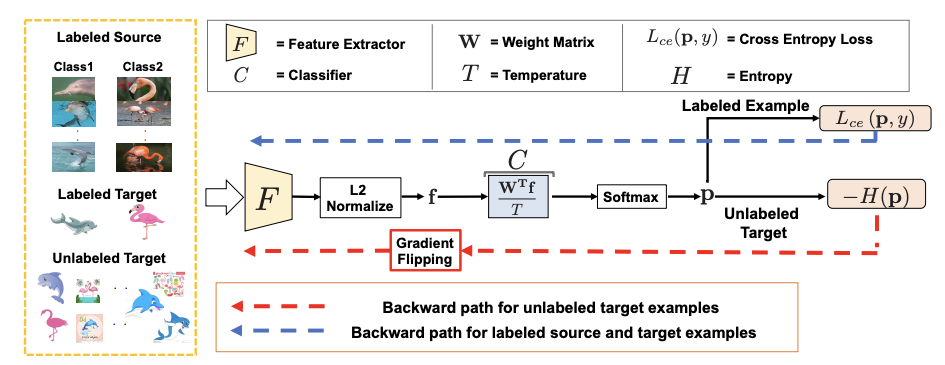
\includegraphics[width=0.48\linewidth]{figures/related_work/MME.png}
    }\hfill
    \subfigure[MHPL样本选择~\cite{MHPL}]{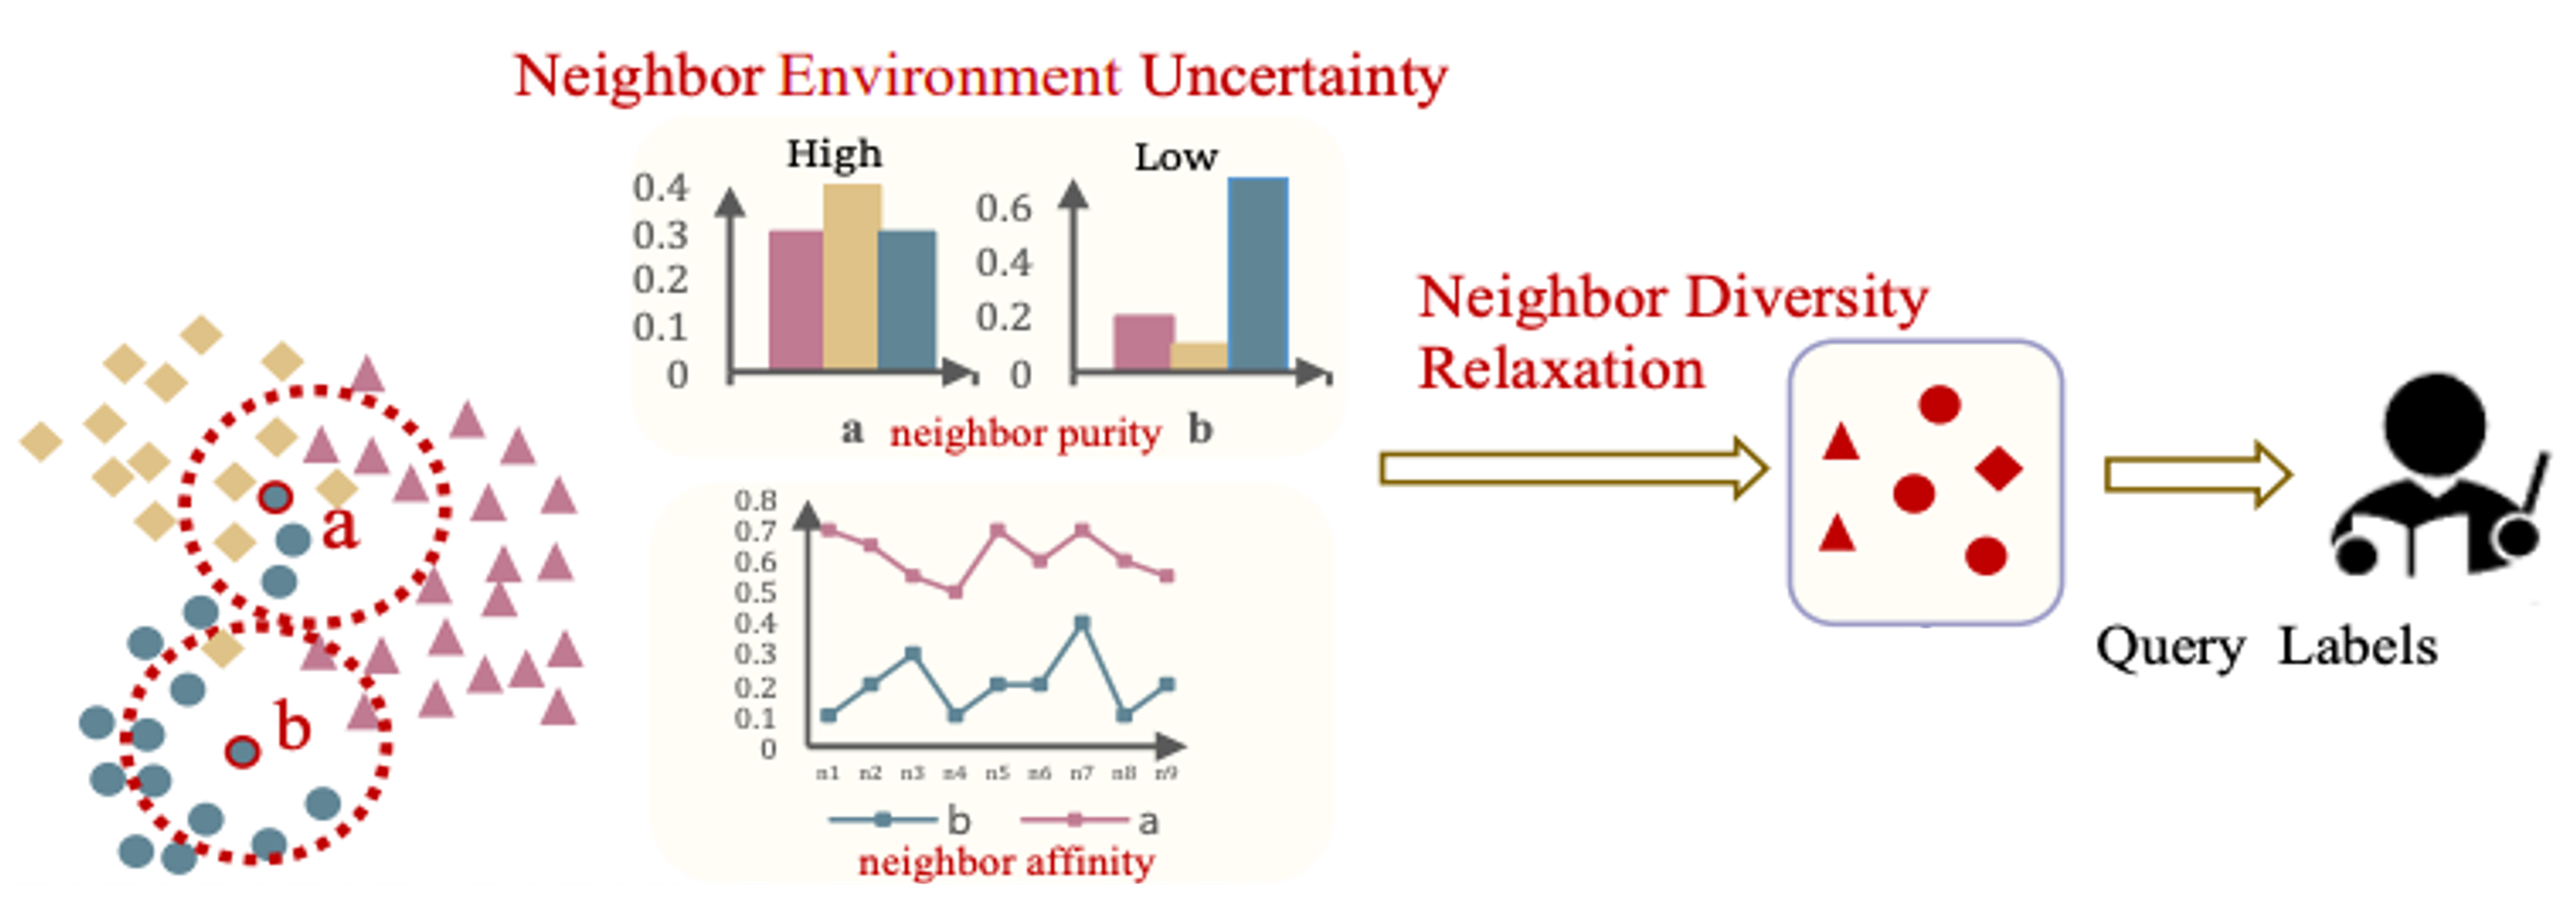
\includegraphics[width=0.48\linewidth]{figures/related_work/MHPL.png}}
    \bicaption[fig:rare_da]{}{少监督域适应代表方法}{Fig.}{Representative methods for limited-supervision domain adaptation}
\end{figure}

半监督SSDA与少样本FSDA域适应设定了有限标注目标样本（每类 1 至 N 个）+ 大量无标注目标样本的标准少监督范式，是少监督域适应方法谱系中最一般化的形式。SSDA 的开创性工作 MME~\cite{saito2019semi} 通过对抗式最小化最大熵同时利用标注与无标注目标样本的边缘分布；后续工作进一步围绕伪标签去噪、对比约束与一致性正则等机制扩展 SSDA 设定下的跨域监督构造。FSDA 进一步收紧至每类仅 1–5 个标注目标样本的极端设定，借助度量学习、元学习或跨域原型对齐缓解极低监督下的过拟合问题~\cite{zhao2021fewshot}。

上述设定下，信息最大化以不同程度地发挥作用。标注预先给定时，它体现为如何充分利用既有的标注与大量无标注目标样本构造有效监督，使有限的先验信息在训练中得到充分兑现；标注由模型筛选时，它还进一步体现为有限的人工标注应投向何处才最为有益。由此，信息最大化在样本选择与模型学习两个环节具有不同的理论刻画。在样本选择层面，Lindley~\cite{lindley1956information} 将一次观测的信息量定义为未知目标函数后验熵的期望下降量；Houlsby 等人~\cite{houlsby2011bayesian} 据此将主动学习的信息增益表示为标签与模型后验之间的互信息。后续研究进一步探讨了信息增益与预测性能的关系~\cite{kirsch2022unifying,bickfordsmith2023prediction,gajjar2023active}。在模型学习层面，Gomes 等人~\cite{gomes2010discriminative} 将预测与标签之间的互信息写为预测边缘熵与条件熵之差；SHOT~\cite{liang2021source} 将相应的信息最大化损失用于域适应自训练，以鼓励预测具有判别性。上述理论分别为选择标注样本和利用目标域数据提供依据，但不能直接等同于目标模型最终获得的迁移收益。

% 将上述界定迁移到本文关注的少监督模型迁移设定还需作两点泛化。其一，待削减的不确定性不再是同分布假设下单一模型的后验不确定性，而是目标域上标注函数的不确定性，由于源模型在目标域存在系统性偏置，这一不确定性需同时从判别性与代表性两个侧面度量。其二，当目标域可用的监督信号来源不止人工标注一条时，单一来源内的信息增益不足以刻画整体监督信息量，还需计入不同来源之间在假设空间上的互补性；这种互补性只有经由学习层面的联合优化与蒸馏传递才能真正转化为目标模型的能力增益，而非停留在样本选择端的样本计数上。本文据此把少监督迁移中的信息最大化界定为：在监督预算约束下，通过样本选择与跨模型协同两方面手段构造互补监督信号，使目标模型经由自训练与蒸馏后对目标域标注函数的逼近能力最强；该界定的量化形式与相应方法在第~\ref{chap:3} 章给出。
在样本选择层面，落实上述准则的经典手段是主动域适应ADA，其核心假设是并非所有目标样本对改善模型的贡献相同，应优先选择对监督信号贡献最大的样本加以标注。具体到可操作的采样策略上，Mathelin 等人~\cite{mathelin2022discrepancy} 从跨域角度出发，区分了模型不确定性与数据不确定性，前者可通过追加标注削减、后者由输入固有噪声决定，从而为不确定性采样与代表性采样这两条互补路径给出了统一的概率解释，并使样本选择层面的信息增益与模型学习层面的能力增益直接挂钩。CLUE~\cite{prabhu2021active}、EADA~\cite{xie2022active}、CA-ADA~\cite{xiao2024category} 等代表性工作将上述样本选择机制与域偏移度量结合，使所选标注样本同时具备对当前模型的不确定性与对目标域分布的代表性。
收紧至“源数据不可访问”这一严格设定，主动无源域适应SFADA的其核心挑战是源数据不可用带来的伪标签噪声放大与外部监督信号缺失。MHPL~\cite{MHPL} 通过联合邻居一致性、个体差异性与域差异性进行样本筛选；ELPT~\cite{li2022source} 优先选择局部结构尚不清晰的样本；SQAdapt~\cite{SQAdapt} 借助数据增强下的预测敏感性度量样本价值；Wang 等人~\cite{wang2023mhpl} 与 Li 等人~\cite{li2023source} 对 SFADA 的设定与挑战给出系统性总结。
% 这类方法主要通过目标样本选择提高有限人工标注的利用效率，而源数据不可访问时，模型学习还需要从其他来源获取互补的语义监督。

需要值得一提的是，视觉—语言基础模型（Vision-Language, ViL）在少监督域适应的跨模型监督中也发挥重要作用，可以作为一路强大的语义监督源。CLIP~\cite{radford2021learning} 与 ALIGN~\cite{jia2021scaling} 凭借海量图文对比学习建立了视觉—语义统一嵌入空间，具备出色的零样本泛化能力；其下游适配策略主要分为三类：提示学习（CoOp~\cite{zhou2022learning}、KgCoOp~\cite{kgcoop}）、参数高效适配器（Tip-Adapter~\cite{Tip-Adapter}）、以及伪标签微调方法（PADCLIP~\cite{lai2023padclip}）。在 UDA 设定下，DAPL~\cite{ge2023domain} 将上下文分解为域无关与域相关部分以解耦语义与域偏置，PADCLIP~\cite{lai2023padclip} 通过调整学习率缓解 CLIP 微调中的灾难性遗忘；在 SFDA 设定下，DIFO~\cite{tang2024source} 通过最大化目标模型与 CLIP 之间的互信息，将 CLIP 的零样本语义知识蒸馏到目标模型。然而现有方法在将 ViL 与目标模型结合时多停留于浅层组合，缺乏理论指导下的双向深度交互机制。

% 综上，面向域泛化场景的跨域不变特征学习指向一个核心问题：如何在迁移机制与骨干架构两条正交维度上协同突破，使模型在“无标注”与“少量标注”两种极端设定下均能实现可靠的跨域不变特征学习。

\subsection{面向类泛化场景的跨域语义关系学习}

开放类别识别是视觉感知的核心需求之一。传统有监督学习在封闭类别 设定下依赖大规模标注数据训练特定分类器，难以扩展至训练时未见 的新类别；跨域语义关系学习旨在突破这一限制——通过挖掘类别 概念之间的语义关联（属性、文本描述、视觉—语言嵌入等侧信息）， 构建对未见类别与新词表具备泛化能力的视觉识别系统。

% 本节按照 从"域偏移下的开类识别"到"开放词表开放世界开类学习"的 递进关系展开：先回顾在域偏移设定下借助语义侧信息识别未知类的 开集域适应与广义零样本工作；进而讨论在无类别边界约束的开放 词表下，利用视觉—语言基础模型与分割基础模型实现像素级开放 词汇分割的最新进展；最后归纳当前研究在统一解码框架深度融合 方面的不足，引出本论文第 4 章的切入角度。

\subparagraph{域偏移下的开类识别}

开集域适应（Open-Set Domain Adaptation, OSDA）将传统域适应从“已见类跨域对齐”扩展到“在跨域迁移中同时识别未知类”，是域偏移下开类识别的代表性设定。与封闭集域适应相比，OSDA 不再假设源—目标域共享同一封闭类别空间，而是承认目标域中可能出现训练时未标注的未知类别，因此要求模型在完成跨域特征对齐的同时，赋予未知类样本独立的“未知”占位判别能力。这一设定广泛存在于工业缺陷检测、医学病灶诊断等真实场景——目标域类别数往往无法被源域类别集完全覆盖。

围绕如何在保留域不变特征的同时刻画未知类，OSDA 衍生出多条技术路线。分离式方法~\cite{liu2021separate} 通过渐进式分离将已知类与未知类样本在特征空间内逐步拉开距离；继承式方法~\cite{kundu2022towards} 提出可继承的源模型结构，使源分类器在目标域未知类新增时仍能保持已见类的判别能力；校正式方法~\cite{li2023adjustment} 引入未知类偏置校正，补偿分类器对未知类样本的判别阈值漂移；关系式方法~\cite{tong2025reserve} 通过挖掘类间语义关系在共享类与未知类之间建立桥梁，利用属性或文本侧信息辅助未知类定位；多域扩展方面，Liu 等人~\cite{liu2025open} 将 OSDA 推广至混合域场景，借助视觉—语言聚焦机制同时应对多个目标域的开放识别需求。在无源数据设定下，Wang 等人~\cite{wang2025active} 将 OSDA 与主动学习结合，在源数据不可访问的严格约束下通过少量人工标注主动识别未知类。

% 与广义零样本学习（Generalized Zero-Shot Learning, GZSL）相比，OSDA 的核心差异在于对未知类的“可见性”假设——GZSL 假设测试阶段可见到所有未见类样本但无对应训练样本，OSDA 则仅假设目标域中含有未知类且不提供任何先验语义信息，因此两者的技术挑战与解决路径存在本质差异。但二者共同体现了“在跨域或跨类别的开放设定下进行识别”这一核心问题。

整体而言，OSDA 工作的核心假设仍是“未知类不可见、但目标域一定含有未知类”，仍依赖于“已知类标签 + 未知类占位”的双分支判别结构，对类别语义侧信息的利用也以已知类内部的语义关联为主，尚未真正引入“任意自然语言描述作为类别”的开放词表机制。这一局限为开放词表识别方向的兴起埋下伏笔。

\subparagraph{开放世界开类学习}

随着视觉—语言基础模型在零样本分类、跨模态检索等任务上 展现出强大的开放语义能力，研究焦点从“有限未知类的开集 识别”推进到“无类别边界约束的开放词表识别（Open-Vocabulary Recognition, OVR）”——即在测试阶段面对任意自然语言描述的 新类别时仍能完成识别。这一开放词表识别能力在检测与分割 两个密集预测任务上分别衍生出开放词汇检测（Open-Vocabulary Detection, OVD）与开放词汇分割（Open-Vocabulary Segmentation, OVS）~\cite{liu2026open}。OVS 要求模型在训练时未见过的新类别上仍能完成像素级识别与分割，其难点由开放词表这一前提直接派生，并集中体现在两个方面：其一，判别依据不得依附于固定的类别索引，模型须能对任意自然语言描述的新类别给出语义响应，而以固定输出维度为前提的判别式模型对此无能为力；其二，新类别在训练阶段没有对应的像素级监督，模型倾向于将目标区域错误归入语义相近的已见类别，掩码边界与类别归属同时失准。

\begin{figure}[!htbp]
    \centering  
    \setlength{\tabcolsep}{0pt}
    \subfigure[两阶段方法OVSeg框架图~\cite{liang2023open}]{
        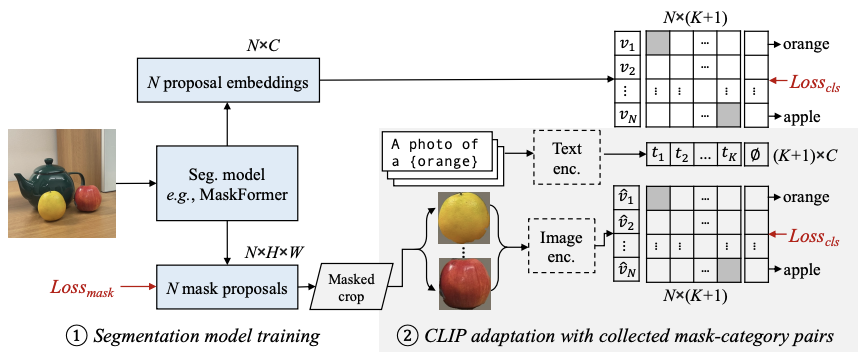
\includegraphics[width=0.48\linewidth]{figures/related_work/ovseg.png}
    }\hfill
    \subfigure[单阶段方法FC-CLIP框架图~\cite{yu2023convolutions}]{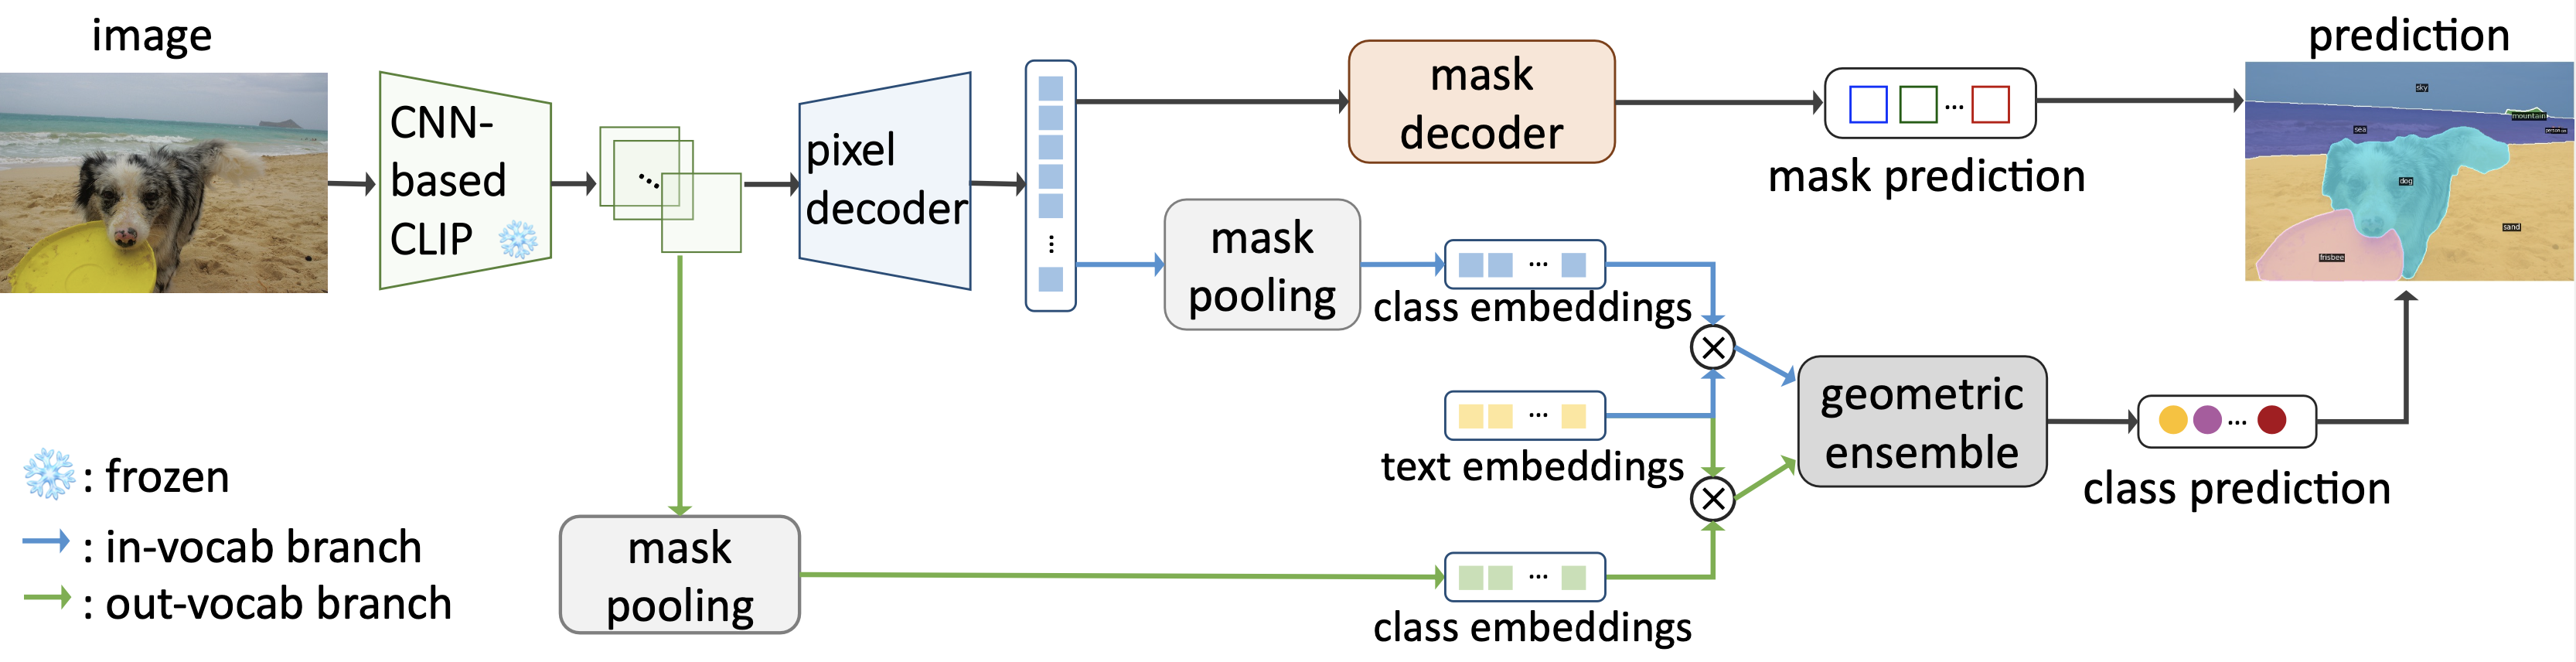
\includegraphics[width=0.48\linewidth]{figures/related_work/fc-clip.png}}
    \bicaption[fig:rare_ovs]{}{代表的开放词表方法}{Fig.}{Representative methods for open-vocabulary methods}
\end{figure}

OVS 方法可沿“先生成掩码再分类”的两阶段路径与“端到端 单阶段”两条主线展开。两阶段方法~\cite{liu2024open,maskclip,xu2022simple,MasQCLIP,liang2023open,chen2023open} 一般先借助额外分割模型生成类别无关掩码提议，再将 ViL 特征与多个掩码提议进行交互以分配语义类别。SCAN~\cite{liu2024open} 通过双流网络联合学习语义无关的掩码与类别嵌入；MaskCLIP~\cite{maskclip} 以类别无关掩码与可学习 mask token 与 CLIP 嵌入交互；OPSNet~\cite{chen2023open} 将 mask query 嵌入与 CLIP 最后一层嵌入结合用于域外类别识别， 并引入 IoU 分支过滤低质量提议；OVSeg~\cite{liang2023open} 通过在大规模开放词汇数据上微调掩码分类器提升密集预测 质量；SimBase~\cite{xu2022simple} 与 MasQCLIP~\cite{MasQCLIP} 进一步简化两阶段流水线并探索 CLIP patch 特征与掩码的对齐。 两阶段方法的主要局限是“先生成、再分类”的串行结构导致 特征不对齐与计算冗余，且对未见类别的掩码质量高度依赖 上游提议模型。

单阶段方法~\cite{yu2023convolutions,wu2024clipself,MGCCL} 将 ViL 模型本身扩展为分割器骨干，端到端地完成密集预测，避免了 掩码提议阶段带来的过拟合风险。FC-CLIP~\cite{yu2023convolutions} 通过在 CLIP 之上引入掩码分类头实现单阶段开放词汇分割； CLIPSelf~\cite{wu2024clipself} 在 CLIP 内部通过自蒸馏提升 patch 级别表征；MGCCL~\cite{MGCCL} 借助多粒度对比学习增强 文本—图像—掩码三方的语义对齐。研究表明，卷积式 CLIP 模型相较 ViT 式 CLIP~\cite{dosovitskiy2021image} 在大输入 分辨率下表现更优，这与其对空间结构的局部归纳偏置密切相关。 然而，CLIP 的 patch 级特征本质上是为图像级识别设计的， 缺乏细粒度的像素级监督，因而在 mask 边界精度与对小目标 的捕捉上存在天然上限：除像素级监督缺失外，patch 网格与对象边界之间的区域级偏置进一步削弱了掩码精度；而推理阶段文本—视觉相似度的计算开销与类别数线性相关，在开放词汇场景下还需配合高效的类别嵌入压缩。针对这些局限，现有缓解思路包括 FC-CLIP 通过卷积 CLIP 提升分辨率适应性、DenseCLIP~\cite{rao2022denseclip} 引入像素—文本密集对齐、CLIPSelf 通过自蒸馏提升 patch 级表征、MGCCL 借助多粒度对比学习联合优化。

视觉—语言基础模型与分割基础模型的融合是 OVS 突破上述困难的关键路径。CLIP 与 ALIGN 在零样本分类、检索、跨模态匹配等任务上展现强大泛化能力；SAM 凭借十亿级分割掩码训练实现任意提示引导的零样本实例分割。SAM 的适应性通过 多种提示策略进一步增强，包括低级视觉提示~\cite{MMRAD}、 弱监督~\cite{ROSE} 等；同期工作 SEEM~\cite{seem} 将空间 提示（点、框、涂鸦、掩码）与文本提示统一到联合图像—文本 表征空间；X-Decoder~\cite{zou2023seg} 通过不同 query 类型 实现任务统一。然而 SAM 本身不输出类别语义，CLIP 又缺乏 像素级密集监督，二者在统一解码框架内的深度融合仍有待 探索。RegionSpot~\cite{yang2024recognize} 通过开放词汇 检测器生成候选框并送入 SAM 完成高质量分割；Open-Vocabulary SAM~\cite{yuan2024open} 借助交互式提示在二十千类上完成 分割与识别。然而上述方法多以“检测器 + SAM”或“CLIP + 分割器” 的松耦合方式组合，掩码质量与类别语义识别之间仍存在错配： SAM 的高质量掩码与 CLIP 的开放语义难以在统一解码框架内 对齐。从松耦合到紧耦合的范式演进中，基础模型融合范式 经历了从外部检测器 + 分割器的两阶段流水线到单阶段 CLIP 骨干 + 分割头的端到端融合、再到跨模型统一解码 的演进。
% 然而上述方法均未在统一解码 框架内充分利用 SAM 的高质量掩码先验，导致掩码质量与 语义识别之间的错配。


\subsection{面向语义理解泛化场景的高阶语义评测}

上一节关注类别词表扩展后模型能否识别并定位未见类别；当目标任务进一步要求模型解释判断依据时，识别结果本身已不足以说明其语义理解是否可靠。多模态大语言模型（Multimodal Large Language Model, MLLM）能够结合图像生成开放式回答，相关评测也从对象、属性和关系的判别，逐步扩展到知识运用与解释生成。然而，答案合理或表述流畅，并不能证明解释中的语义结论得到了视觉证据支持。对这一差别的考察需要先了解通用基准如何测量感知与推理，再进入对证据依赖更强的具体任务。艺术情感理解正是此类任务的代表：情感判断往往涉及构图、色彩等多种线索，评测既要考察模型给出何种判断，也要检验其如何将判断与可见线索关联。

通用多模态基准为区分不同视觉能力提供了起点。MMBench~\cite{mmbench2023} 将感知与推理细化为多个能力维度，通过选择题比较模型在属性识别、空间关系等任务上的表现；SEED-Bench~\cite{seedbench2024} 进一步覆盖图像与视频理解，使评测对象从静态画面扩展至时间信息。ScienceQA~\cite{lu2022scienceqa} 和 MMMU~\cite{yue2024mmmu} 则将科学知识、多学科材料与图像共同纳入问答任务，提高了对知识运用和复杂推理的要求。这些基准采用不同的任务划分，它们能够揭示模型在哪类题目上答对或答错，但在以最终答案为主要评分对象时，正确答案仍不足以单独证明模型生成的解释引用了相关视觉证据。

% 图~\ref{fig:related_benchmarks} 对照展示了通用能力基准与图像情感基准的任务形式。

对开放式回答的评测进一步将注意力从答案延伸到生成内容。GAVIE~\cite{liu2024gavie} 借助模型辅助评判考察视觉指令回答的质量与幻觉；FaithScore~\cite{jing2024faithscore} 将生成描述拆解为可核验的原子事实，再检查这些事实是否与输入图像一致。前者扩展了开放回答的评判方式，后者提供了比整体流畅度更细的事实一致性度量。不过，描述中的对象和属性均属实，也不意味着模型已经说明它们为何共同支持某种抽象语义判断。面向解释本身，VQA-X~\cite{park2018multimodal} 同时收集文字理由和视觉指向，表明回答、理由及其指向的图像区域可以分别考察；其任务主要围绕视觉问答中的决策解释。


\begin{figure}[!htbp]
    \centering  
    \setlength{\tabcolsep}{0pt}
    \subfigure[视觉-语言模型多模态能力评测基准MMBench~\cite{mmbench2023}]{
        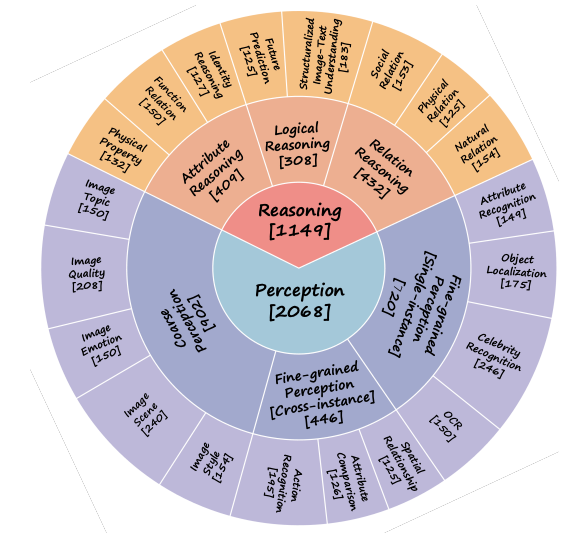
\includegraphics[width=0.48\linewidth]{figures/related_work/mmbench.png}
    }\hfill
    \subfigure[图像情感评测基准EEmo-Bench~\cite{eemobench2025}]{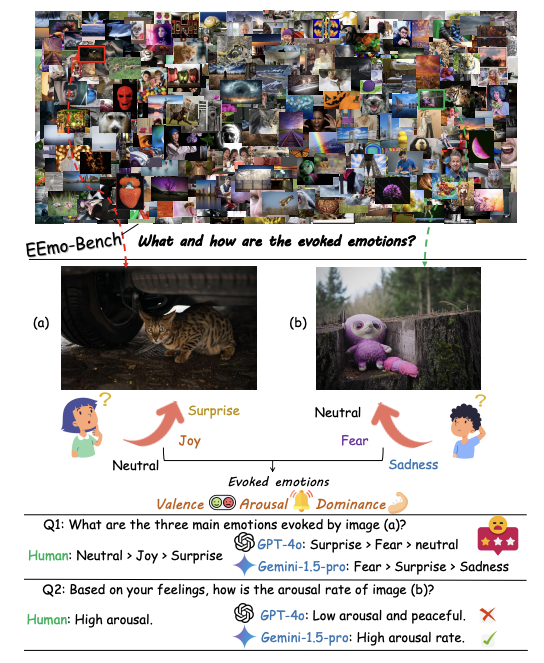
\includegraphics[width=0.38\linewidth]{figures/related_work/EEmo-Bench.png}}
    \bicaption[fig:related_benchmarks]{}{代表性的语义评测基准}{Fig.}{Representative benchmarks for semantic evaluation}
\end{figure}

艺术情感理解需要同时关注作品传达了何种情感，以及观看者依据哪些视觉线索作出判断。图~\ref{fig:related_benchmarks} 对照展示了通用能力基准与图像情感基准的任务形式。作品的情感效果可能来自对象内容，也可能来自色彩、光照、构图和笔触；不同观看者对同一作品的感受也未必一致。ArtEmis~\cite{achlioptas2021artemis} 为艺术作品收集情感归因及其文字解释，记录观看者的情感反应与理由；EmoSet~\cite{yang2023emoset} 在情感类别之外标注亮度、色彩、场景、对象、表情和动作等属性，为分析视觉内容与情感判断的关系提供了依据。效价、唤醒度与支配度等连续维度还可描述情感状态及强度差异~\cite{you2016building}。这些资源分别从解释、视觉属性和情感维度提供研究材料，但标注对象与粒度不同，尚需进一步组织为能够区分模型感知、情感判断与解释能力的评测任务。

视觉线索的定位也已有专门研究，而非完全空白。APOLO~\cite{chen2024stimuli} 将艺术作品中引发特定情感的区域标注为像素级刺激线索，使研究者能够评价模型是否找到了相关位置。这与 ArtEmis 的自然语言解释形成互补：前者强调证据位于何处，后者记录观看者如何表述感受及其理由。但定位到某个区域，并不能自动判断模型是否正确解释了该区域的形式属性与情感含义之间的关系；反过来，一段合理的文字解释也未必精确指向相关视觉区域。因此，情感归因需要同时关注线索识别、语义关联与解释质量。

在上述情感标注与视觉线索研究的基础上，面向 MLLM 的工作进一步将情感理解组织为可比较的评测任务。EEmo-Bench~\cite{eemobench2025} 涵盖单图感知、情感排序、描述与评估，并通过配对图像考察模型对情感差异的辨别能力，表明单一分类准确率不足以概括情感理解水平。相邻的美学评测研究也逐步引入细粒度属性与开放式描述：AesExpert~\cite{aesexpert2024} 构建多类型美学评价指令，ArtiMuse~\cite{cao2025artimuse} 结合属性分析、专家式评述与整体评分。不过，美学质量评价与情感归因的目标并不相同；即使模型能够给出合理的情感描述，仍需进一步判断其解释是否准确关联了作品中的具体视觉线索。

综上，已有研究分别推进了通用问答、事实一致性、视觉指向、情感标注和美学评论的评测。真正需要进一步衔接的是三种可区分的判断：模型是否识别了作品中的相关线索，能否据此作出情感判断，以及能否在解释中准确建立线索与判断的联系。仅比较最终情感标签、文字流畅度或证据区域，均难以单独定位这一链条中的失效环节。本文在第五章以艺术情感推理为目标任务，将感知、情感、推理和描述设计为相互补充的评测维度，结合单图与配对任务刻画 MLLM 既有能力向高阶语义任务延伸时的适用范围；评测旨在诊断能力边界，而非通过评测本身提升模型性能。

\subsection{现有方法的主要问题}

\noindent\textbf{（1）现有无监督方法在跨域分布偏移下的不确定性建模上存在瓶颈}

无标签目标域中的迁移不确定性同时涉及目标预测的可靠性和特征表征的稳定性。现有伪标签自训练方法往往依据预测置信度或固定阈值筛选样本；当源模型在目标域发生系统性偏移时，高置信预测也可能出错，筛选结果因而难以准确反映伪标签的可靠程度。另一方面，骨干网络可能保留源域纹理、背景或空间共现等域特异性线索，使目标特征的类别结构发生偏移，并进一步影响伪标签生成。两类问题在迭代训练中相互作用：不稳定的表征增加错误伪标签，错误监督又可能强化原有的特征偏移。因此，现有方法仍需解决如何在不访问源数据的条件下评估目标样本的监督可靠性，并同时抑制骨干表征中的虚假相关性，以减轻自训练过程中的误差累积。

\noindent\textbf{（2）现有少监督方法在信息驱动的样本挖掘与跨模态协同上存在不足}

在目标域仅有少量标注样本可用的稀缺监督条件下，如何拓展监督信号的来源与协同深度，是模型迁移设定下的另一关键研究问题。视觉—语言等大模型凭借大规模跨模态预训练获得了对开放语义的零样本判别能力，其预测不依赖源域分布，能够为目标样本提供与源模型假设空间互补的语义判断信号，这对缓解源模型在目标域上的预测偏置、扩展稀缺标注预算下的监督信息量具有重要价值。然而现有方法在样本选择与跨模态协同两个环节均缺乏对多模态预训练模型监督信号的系统探索，未能建立视觉—语言模型与源模型在信息驱动采样与双向深度协同层面的严谨理论框架。因此，如何实现视觉—语言模型与源模型在信息驱动采样与双向深度协同层面的协同，是模型迁移研究需要解决的关键问题。

\noindent\textbf{（3）现有跨类泛化方法在多流语义对齐与空间定位上探索不足}

视觉—语言模型与分割基础模型分别提供了开放词表的语义锚点与像素级空间定位能力，二者的协同融合被视为突破该问题的关键路径。然而现有方法在多流语义对齐与空间定位两个层面均存在不足：在多流语义对齐层面，两阶段与单阶段方案均难以在统一框架下实现掩码生成与开放词汇识别之间的深度协同；在空间定位层面，现有方案难以同时兼顾对像素级对齐的精细建模与对未见类别的掩码质量，致使对长尾与未见类别的细粒度识别能力受限。因此，如何在统一解码框架内深度融合分割基础模型的空间定位能力与视觉—语言模型的开放词汇语义能力，通过多流语义对齐与空间定位的协同优化实现对长尾与未见类别的泛化，是跨类泛化研究亟待解决的核心问题。

\noindent\textbf{（4）现有语义理解基准在证据锚定与评测维度建模上存在缺口}

语义理解要求模型在开放式语义理解的基础上具备对抽象语义与文化背景的稳健推理能力。语义类评测相对事实类评测具有显著的特殊性：受主观性、抽象性与文化语境三重影响，语义类内容的可靠解释难以被“事实正确性”或“流畅表述”等单一维度度量。已有研究分别提供了情感解释文本、视觉刺激区域、多维情感任务和美学属性分析，但这些评测对象尚未充分贯通，因而难以区分模型是遗漏了相关线索、错误地建立了线索与情感的关联，还是仅在文字表述上缺乏证据支撑。因此，如何构建兼具结构化诊断能力与开放式评分灵活性的多层级评测基准，是语义理解评测需要进一步解决的问题。

\section{本文的主要研究内容及组织结构}

\subsection{本文的研究内容}

前文表明，训练与目标条件之间的差异既可能改变样本分布和类别范围，也可能提高目标任务对语义解释的要求。针对数据分布与类别词表变化，本文研究如何利用有限的目标侧信息和预训练先验改善模型的迁移表现；针对语义理解要求的提高，本文研究如何在不更新模型的条件下评估既有能力的适用范围。两类工作分别从能力提升和能力评测回应多泛化场景下的模型迁移问题，具体归纳为以下四个研究问题。


\noindent\textbf{（1）无监督模型迁移的不确定性抑制问题}

无监督模型迁移中的不确定性源于源模型所学判别依据与目标域数据之间的失配，并在伪标签自训练过程中持续演化：域特异性线索使目标表征和预测偏移，错误预测被赋予伪标签后又作为监督信号参与更新，进一步放大初始偏差。本文围绕这一不确定性的产生、估计与传播开展研究。首先，以目标样本的邻域结构估计伪标签可靠性，识别并抑制错误监督在判别层的累积；其次，考察骨干网络对跨通道关系和背景空间共现的建模方式，削弱域特异性虚假相关对表征及后续伪标签生成的影响。由此，本文将可靠监督信号的构建与跨域稳定表征的学习联系起来，研究二者如何共同抑制无标签适应过程中的误差反馈。

\noindent\textbf{（2）少监督模型迁移的信息最大化问题}

在目标域标注稀缺的条件下，少监督模型迁移需要解决的核心问题是：有限的监督信息能否有效约束目标域中的预测误差，使模型在分布偏移下仍获得可靠的判别能力。这里的信息最大化是固定监督预算下提高目标域学习收益的研究目标。现有方法分别从标注样本利用和目标模型训练等角度提高迁移性能，但对有限监督如何覆盖目标域差异、如何转化为目标模型能力仍缺乏统一刻画。本文据此分析标注集合的覆盖缺额及补充监督与目标模型之间的差异，并进一步研究主动样本选择和跨模型协同学习，使有限标注与互补语义知识共同改善目标域预测。

\noindent\textbf{（3）模型泛化的多模态类别先验挖掘问题}

跨类泛化的核心要求是模型对训练阶段未见过的新颖类别保持识别能力，其关键在于系统挖掘并融合多源类别先验。现有方法多沿单一先验源或粗粒度拼接展开，缺乏在不同网络层级上的双向注入与协同机制。本文从多层级协同融合与双向耦合两个维度展开：在多层级协同融合层面，使空间定位与开放词汇语义两类先验在不同网络深度上交叉作用而非简单串接；在双向耦合层面，使两类先验在网络前向推理中相互增强而非单向辅助，从而在多个细粒度识别任务上取得优于现有方法的性能。

\noindent\textbf{（4）多维度语义理解基准制定问题}

现有评测已分别涉及情感标签、视觉属性、解释文本与刺激区域，但缺少在同一任务体系中追踪感知线索、情感判断及证据化解释之间关系的诊断方式。本文围绕证据化解释与多维度诊断两个要素展开：在证据化解释层面，区分有视觉依据的情感解释与缺乏相关依据的流畅表述；在多维度诊断层面，将语义理解能力拆解为互补任务，并结合结构化题目与开放式评分定位具体能力缺口。

\subsection{本文的组织结构}

\begin{figure}[!htbp]
 \centering
 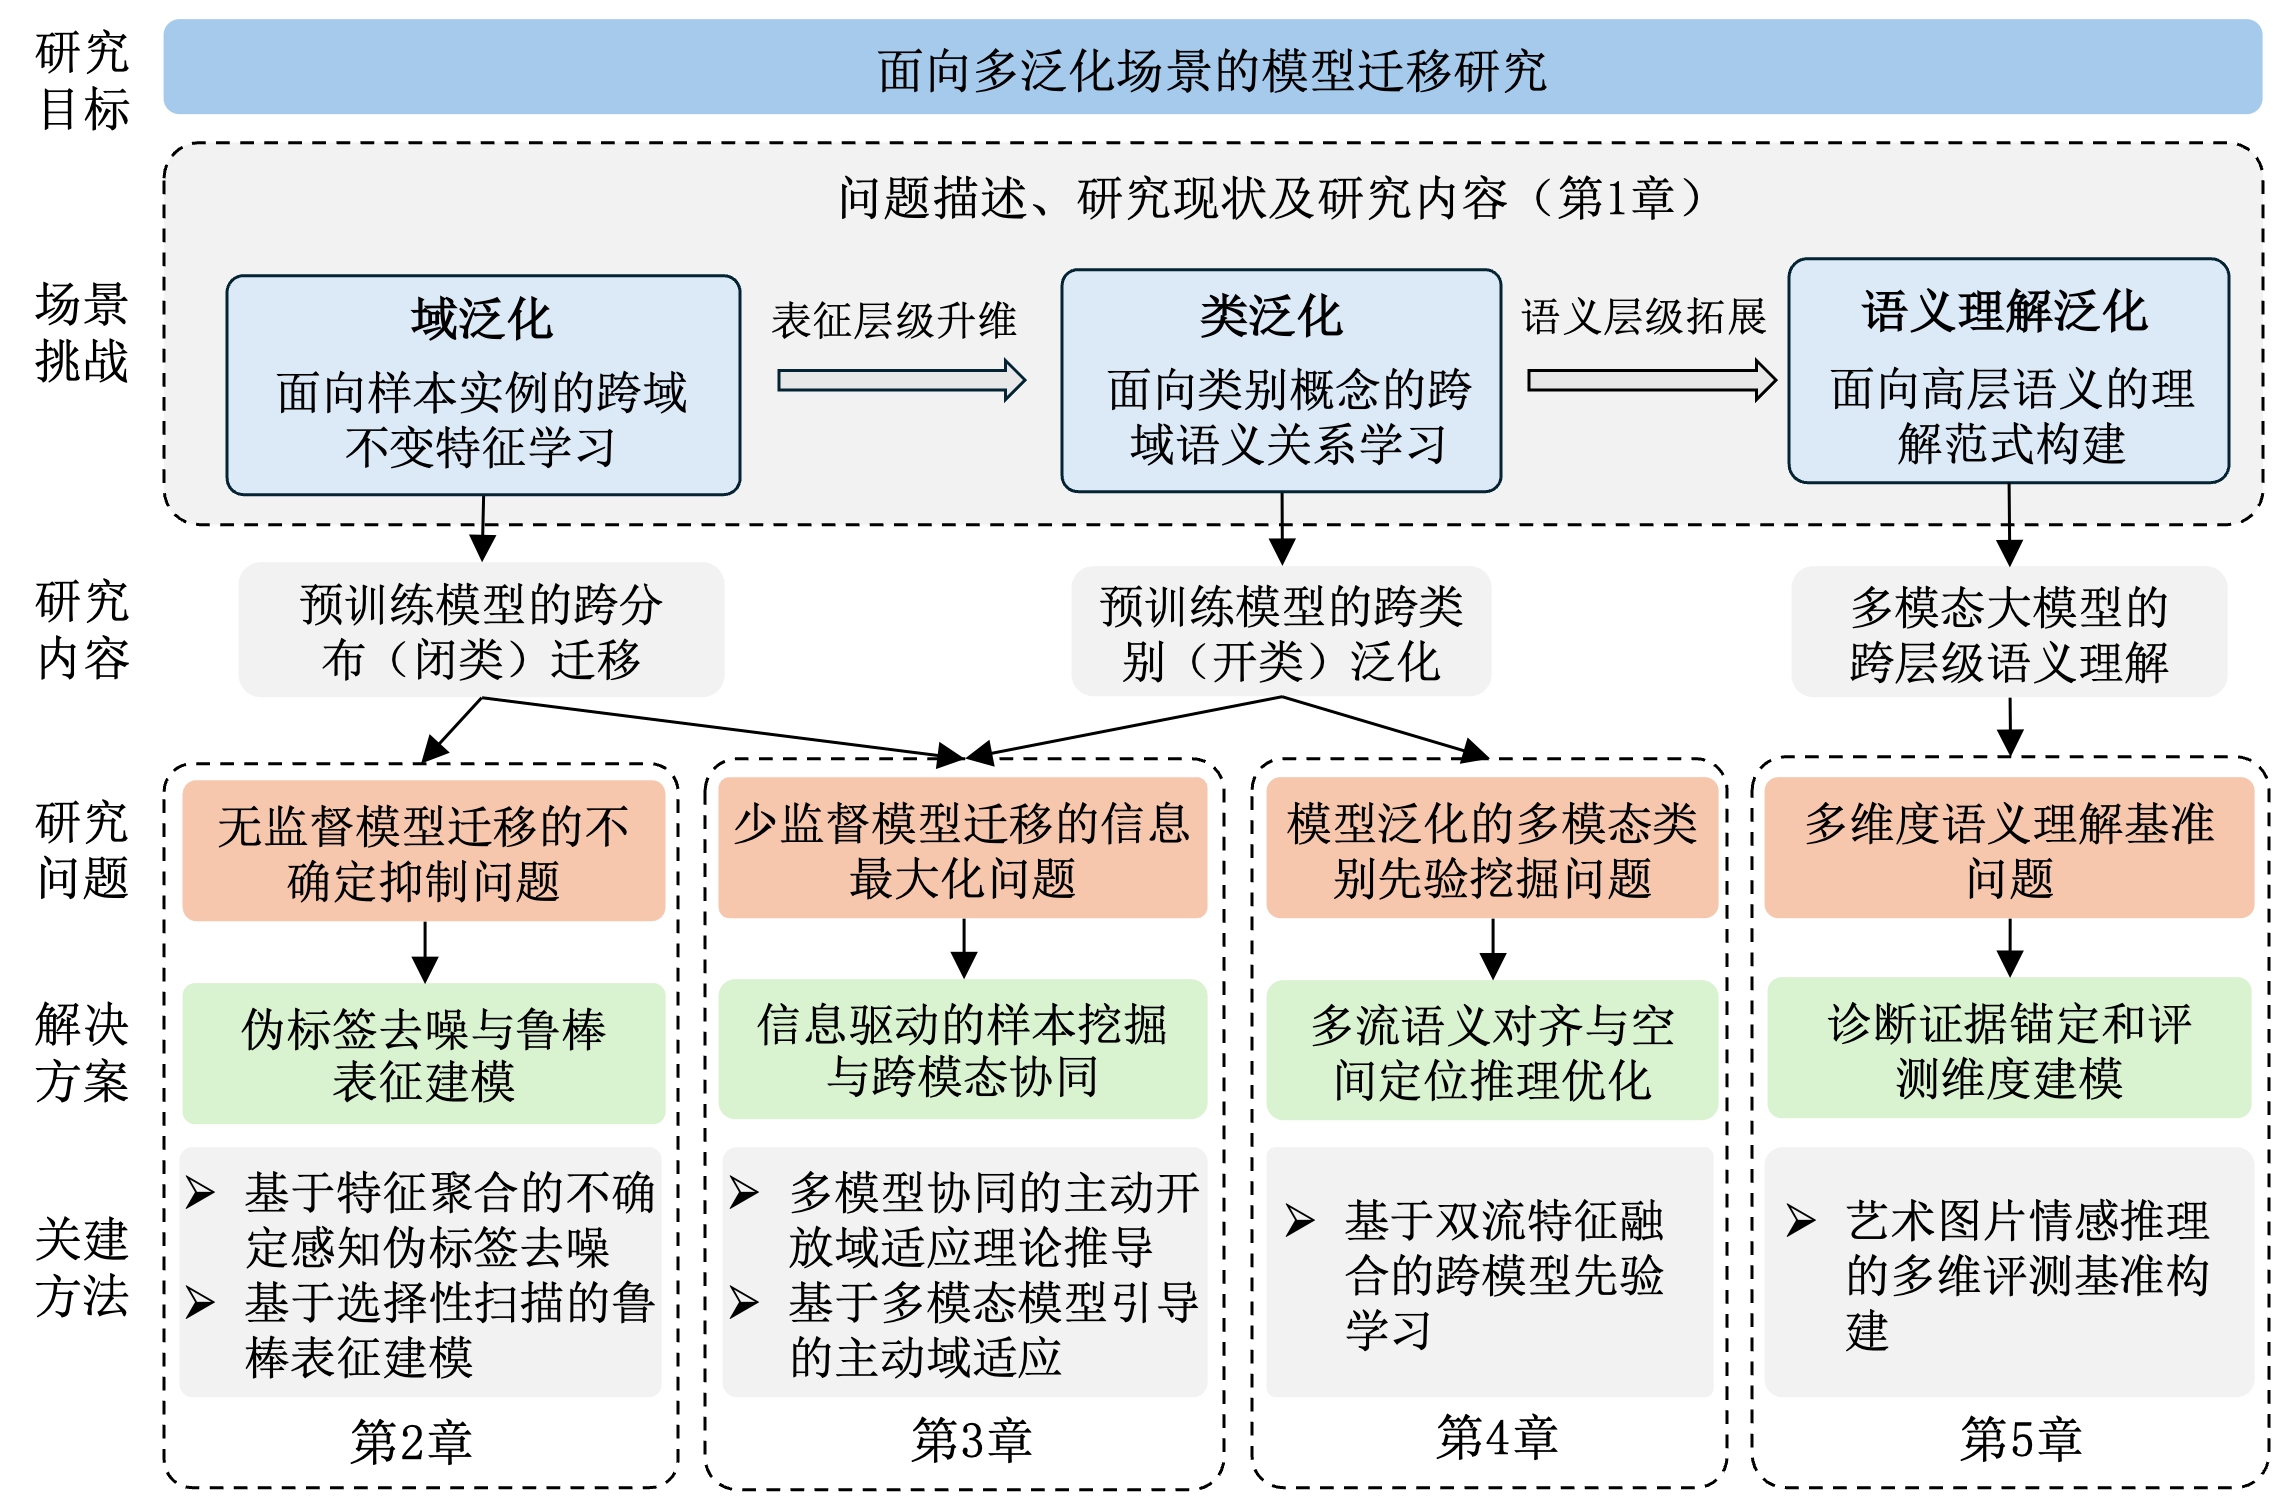
\includegraphics[width=1.\textwidth]{figures/frame.png}
 \bicaption[fig:research_map]{}{面向多泛化场景的模型迁移研究框架}{Fig.}{Research framework of model transfer across multiple generalization scenarios.}
\end{figure}


本文的研究目标是面向多泛化场景的模型迁移研究。如图~\ref{fig:research_map}所示，本文以数据分布、类别词表和语义层次的变化为主线，将研究内容组织为域泛化、类泛化和语义理解泛化三个递进层次。三个层次分别对应预训练模型的跨分布闭类迁移、跨类别开类泛化，以及多模态大语言模型的跨层级语义理解。
% 本文主要研究内容及各章节关系如图~\ref{fig:research_map}所示。

首先，本文面向样本实例的跨域不变特征学习，研究无监督模型迁移中的不确定性抑制问题。无源域适应中，源模型对域特异性线索的依赖可能使目标域表征与预测发生偏移；由此产生的错误伪标签又会在自训练中传播，进一步放大迁移误差。针对伪标签监督的可靠性问题，本文提出基于特征聚合的不确定性感知伪标签去噪方法 UPA，利用邻域一致性估计样本级伪标签可靠性，并结合类别感知对比学习抑制噪声传播；针对表征建模中的虚假相关性问题，提出基于选择性扫描的迁移方法 SfMamba，通过通道级视觉状态空间模块与语义一致性打乱策略增强跨域表征的稳定性。两项工作分别作用于监督信号和特征表征环节，在统一自训练框架下共同减轻迁移误差的累积。
在此基础上，面向稀缺标注预算下跨模型协同监督不足的问题，针对源模型与视觉—语言模型假设空间层面的信息对齐与知识迁移问题，提出基于多模态基础模型引导的双主动域适应方法 DAMF，将视觉—语言模型作为目标样本与源假设空间之间的互补语义监督信号，通过双聚焦样本选择与交替蒸馏实现两类模型在开放集假设空间的双向深度协同。

面向跨类泛化这种面向类别概念的跨语义关系学习，首先针对开放集无源域适应中已知类别与未知类别难以同时兼顾的问题，利用视觉—语言模型在自然语言空间的零样本识别能力指导目标域已知类的判别建模，进一步通过不确定性感知的开放集校准机制实现对未知类别样本的可靠识别；其次针对开放词汇分割中掩码质量与类别语义识别之间的错配问题，视觉定位模型擅长像素级定位但缺乏语义泛化能力、语义—语言模型具备零样本识别能力但特征空间偏全局且边界粗糙，提出跨模型先验融合的开放词汇分割方法 CMPF，将定位模型的空间先验与语义模型的类别先验在统一解码框架内交叉融合，实现对未见类别的稳定识别。

进一步的，面向多模态多维度的情感评测的基准构建需求，针对多维度语义理解基准制定问题，构建AER-Bench，建立从低层视觉线索到高层情感推理的结构化诊断框架，将艺术情感理解拆解为感知维度、情感与 VAD、基于证据的推理、情感描述四个互补层级并模板化生成单图/配对结构化题目，通过确定性指标与基于大语言模型的细粒度评分相结合的混合协议，对代表性多模态大语言模型在艺术情感推理上的能力进行系统评测，揭示其在视觉证据锚定、感知—情感映射与情感解释一致性上的系统性缺陷。

相关研究沿图~\ref{fig:research_map}所示的表征层级升维与语义层级拓展展开：前两层以适应方法提升跨分布与跨类别能力，第三层以多维评测刻画跨层级语义理解的能力边界，共同构成本文对多泛化场景下模型迁移的研究。
% Local Variables:
% TeX-master: "../thesis"
% TeX-engine: xetex
% End:
